% *********************************************************************
% © 2021–2024 Jeremy Sylvestre
%
% Permission is granted to copy, distribute and/or modify this document
% under the terms of the GNU Free Documentation License, Version 1.3 or
% any later version published by the Free Software Foundation; with no
% Invariant Sections, no Front-Cover Texts, and no Back-Cover Texts. A
% copy of the license is included in the appendix entitled “GNU Free
% Documentation License” that appears in the output document of this
% PreTeXt source code. All trademarks™ are the registered® marks of
% their respective owners.
%
% *********************************************************************

\newcommand*{\xmin}{-2.25}
\newcommand*{\xmax}{2.25}
\newcommand*{\ymin}{-1.25}
\newcommand*{\ymax}{1.25}

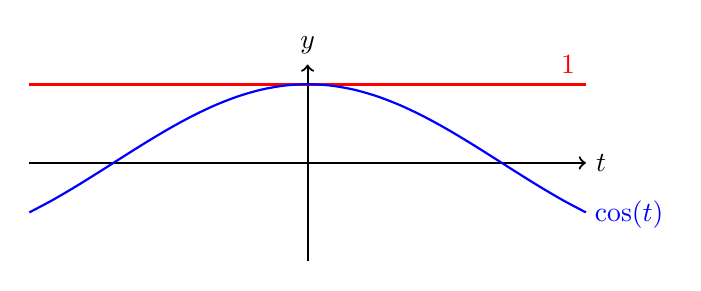
\begin{tikzpicture}
[
	closedpt/.style={circle,draw,fill,inner sep=0pt,minimum size=4pt},
	openpt/.style={circle,draw,inner sep=0pt,minimum size=4pt},
	xscale=1.570796327
]

	% axes
	\draw[->,thick] (\xmin,0) -- (\xmax,0) node[right] {$t$};
	\draw[->,thick] (0,\ymin) -- (0,\ymax) node[above] {$y$};

	\draw[red, very thick] (\xmin,1) -- (\xmax,1) node[above left] {$1$};

	\draw[blue,thick,domain=\xmin:\xmax,smooth] plot (\x,{cos(deg(\x))});

	% \draw[red, very thick,domain=-1.8:1.8,smooth] plot (\x,{1 - \x * \x / 2});

	\node[blue] at (2.6,-0.66) {$\cos(t)$};
	% \node[red,left] at (1.66,-0.66) {$1 - t^2/2$};

\end{tikzpicture}
